%\usepackage[pdftex]{graphicx} % For including graphics N.B. pdftex graphics 

\begin{itemize}
	\item Chen 2015 (Theory of wormlike polymers) discusses the NI transition density
\end{itemize}

The use of neural networks as a tool in condensed matter research has seen a growth in popularity. One of the marvels and advantages of this technique is how little statistical-physics information (energies, order parameters, etc.) is needed for the classification of states or the pinpointing of critical physical parameters.
Even relatively simple neural network models can learn phase-transition temperatures, order parameters, and quantum-state tomography, from the information of a simple feature such as position coordinates in an off-lattice model or the location and value of spins in an Ising model. This could all be done without any knowledge of the original Hamiltonian or interaction potential energies \cite{torlaiboltzmann,carras,wei,wetzel,torlai,morningstar,beach}.


\begin{figure*}[!t]
	\centering
	\begin{minipage}[t]{0.25\textwidth}
		\centering
		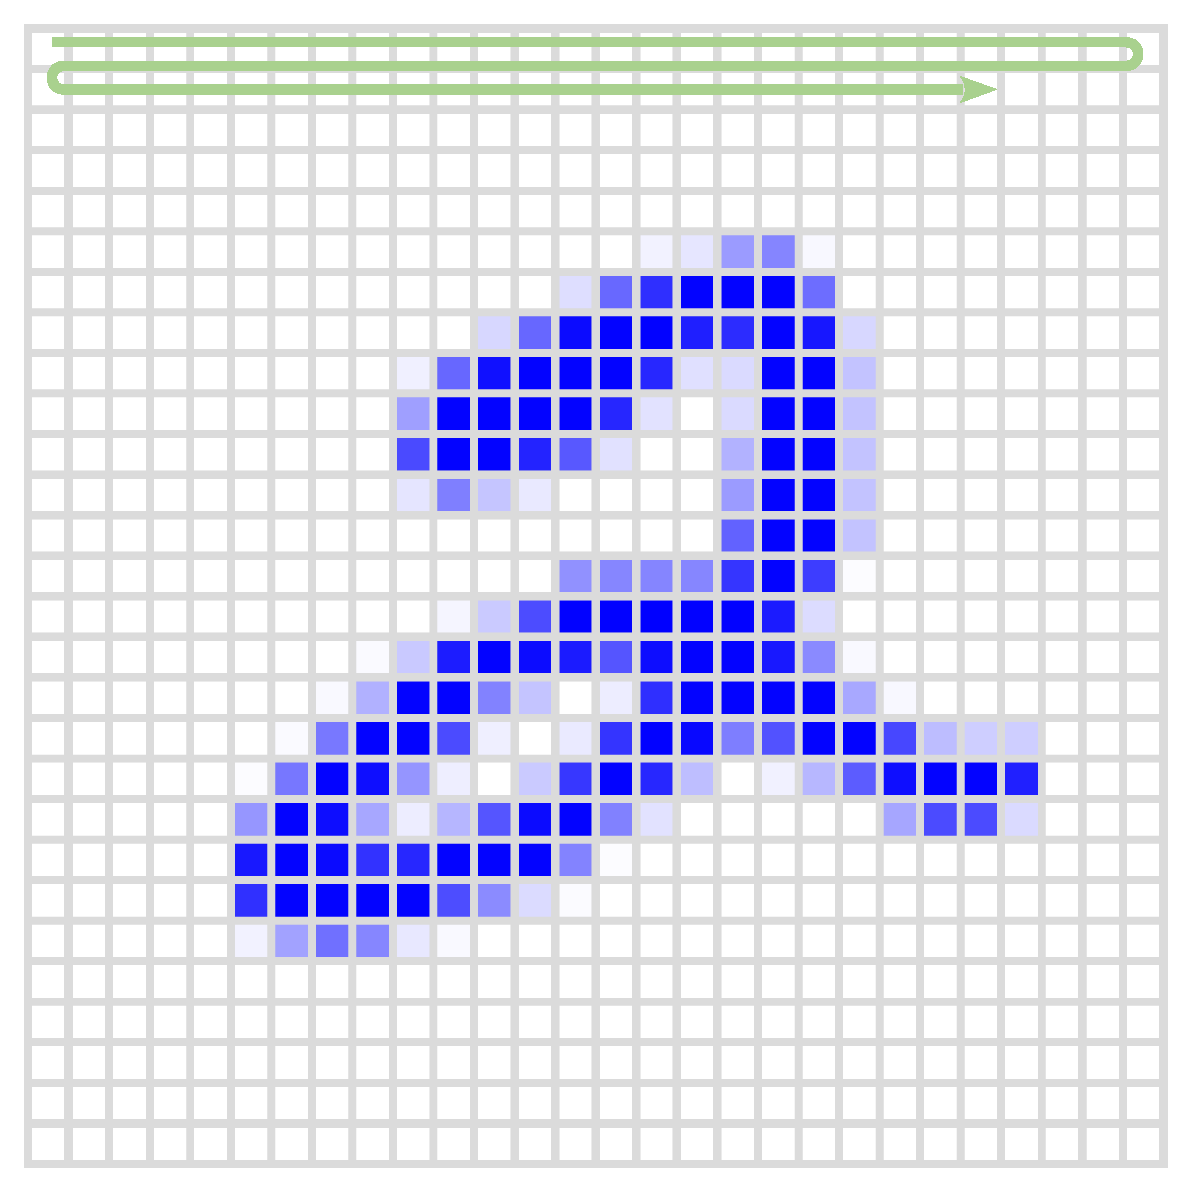
\includegraphics[width=0.9\columnwidth]{./figs/FIG1A.eps}\\
		(a)\\ \vspace{0.5cm}
		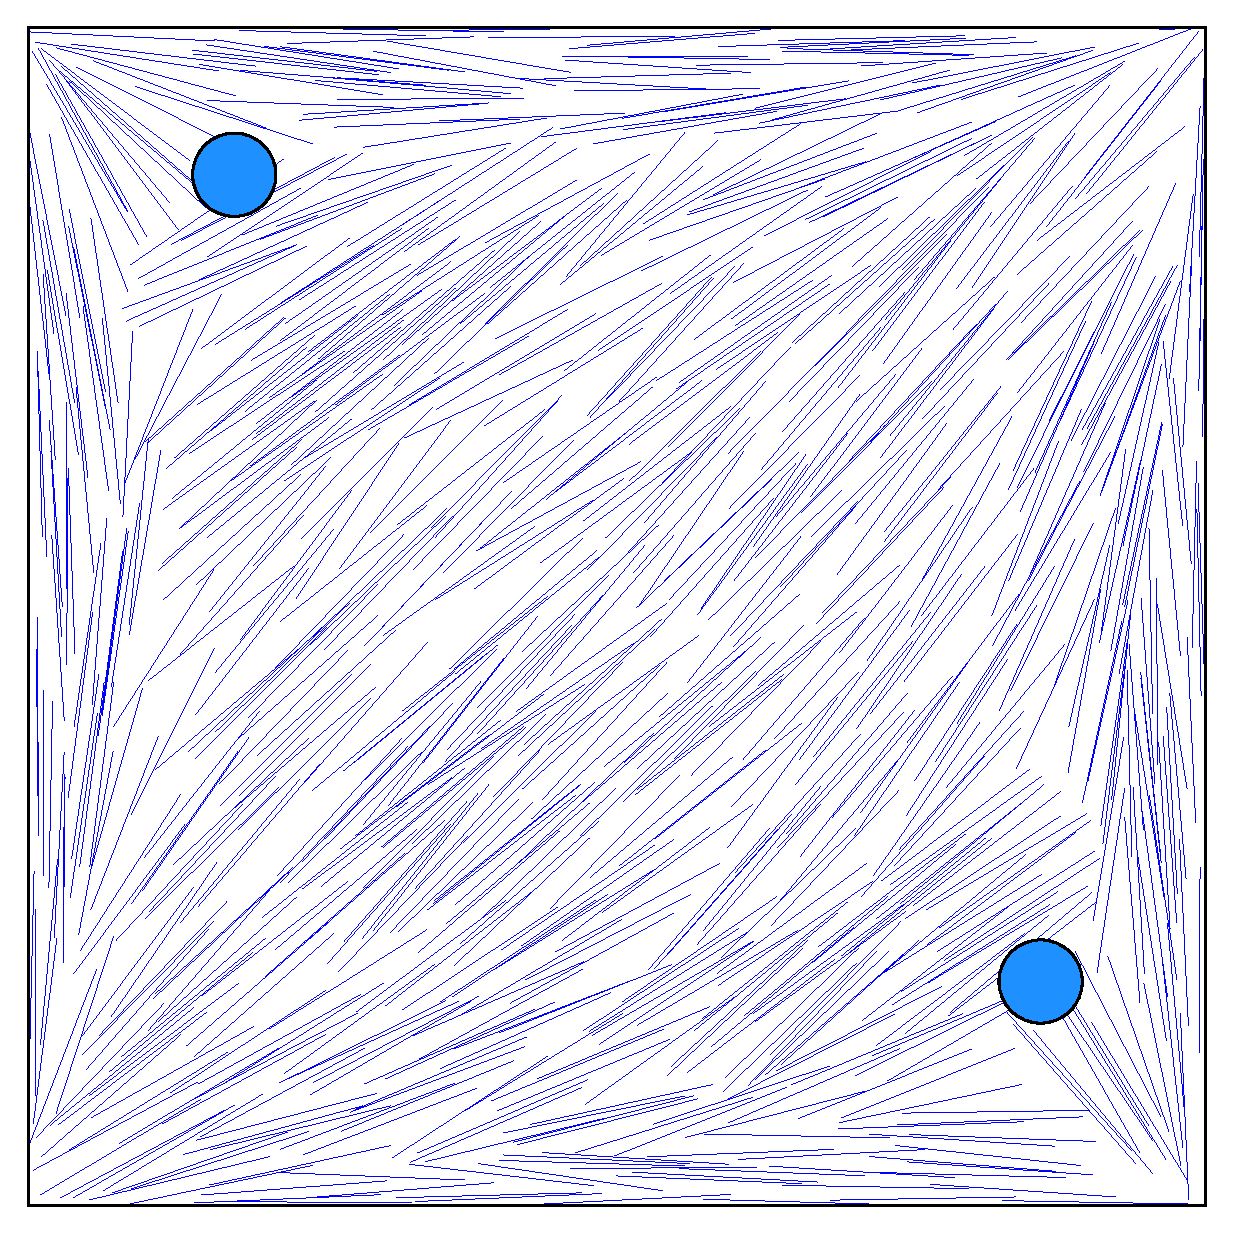
\includegraphics[width=0.9\columnwidth]{./figs/FIG1E.eps}\\
		(e)
	\end{minipage}%
	\begin{minipage}[t]{0.25\textwidth}
		\centering
		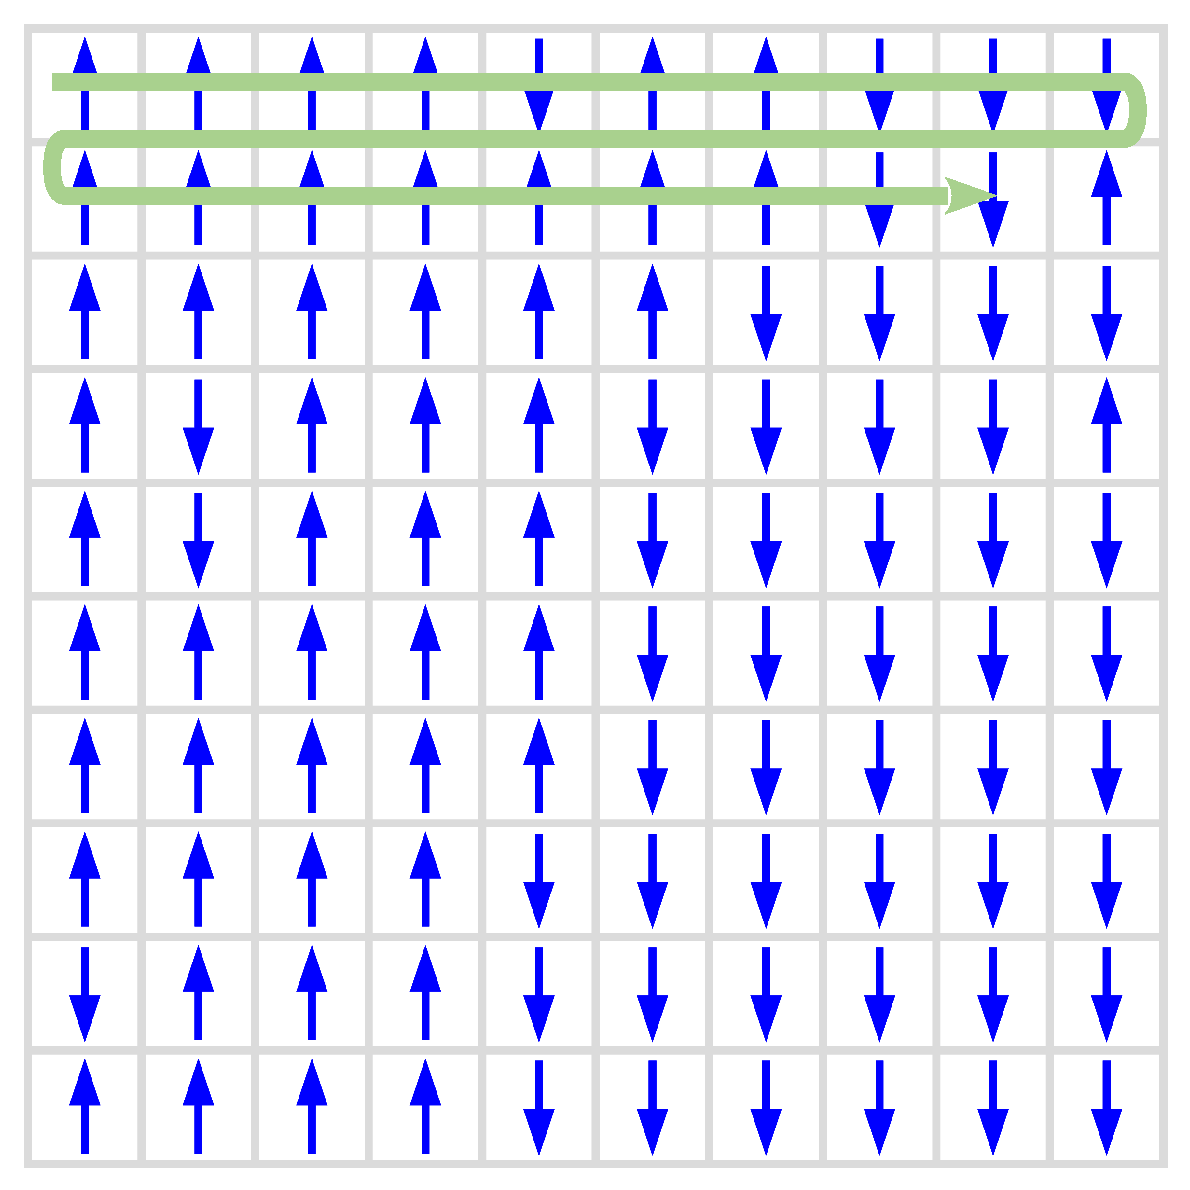
\includegraphics[width=0.9\columnwidth]{./figs/FIG1B.eps}\\
		(b)\\ \vspace{0.5cm}
		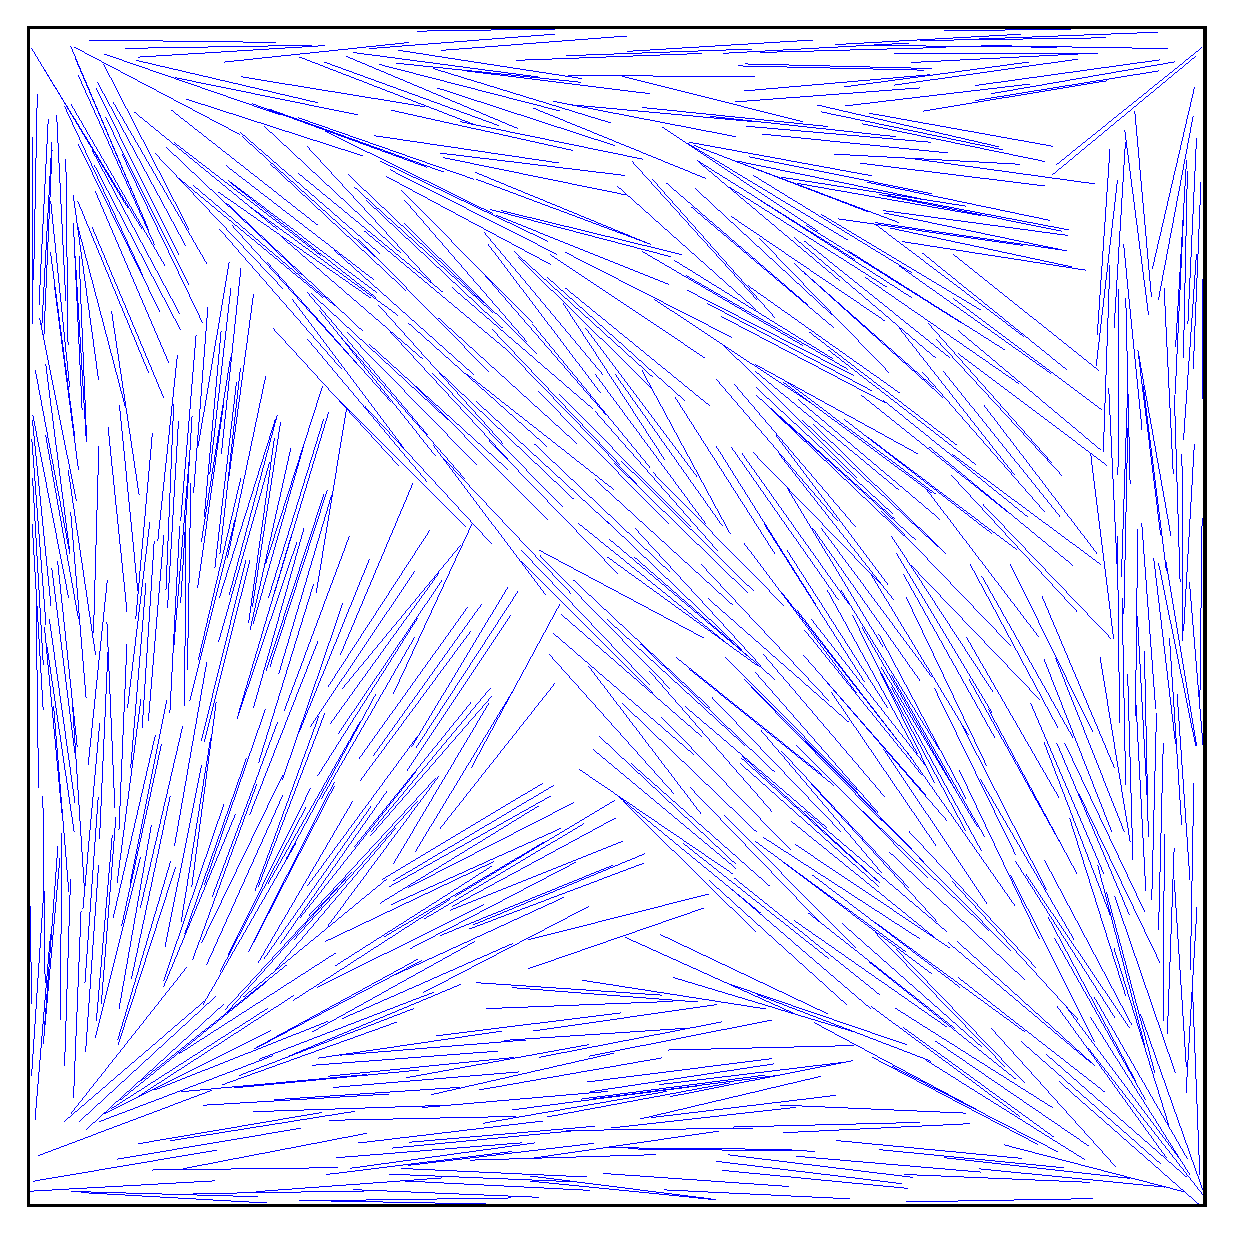
\includegraphics[width=0.9\columnwidth]{./figs/FIG1F.eps}\\
		(f)
	\end{minipage}%
	\begin{minipage}[t]{0.25\textwidth}
		\centering
		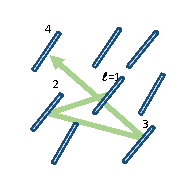
\includegraphics[width=0.9\columnwidth]{./figs/FIG1C.eps}\\
		(c)\\ \vspace{0.5cm}
		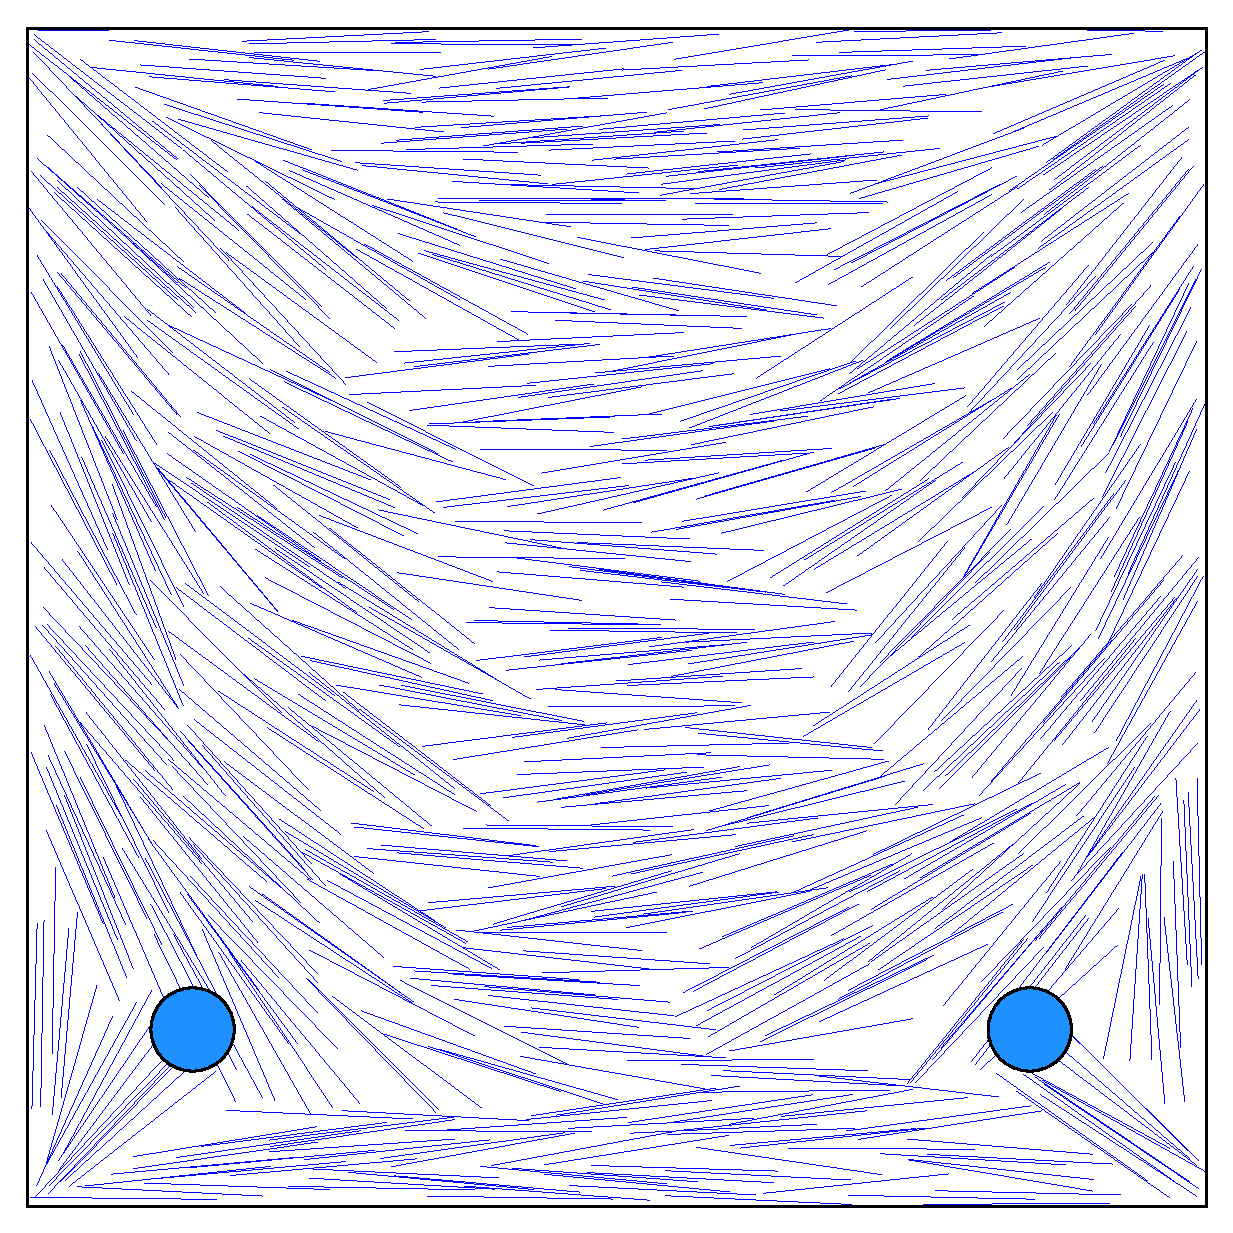
\includegraphics[width=0.9\columnwidth]{./figs/FIG1G.eps}\\
		(g)
	\end{minipage}%
	\begin{minipage}[t]{0.25\textwidth}
		\centering
		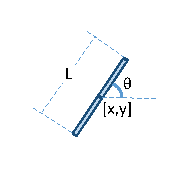
\includegraphics[width=0.9\columnwidth]{./figs/FIG1D.eps}\\
		(d)\\ \vspace{0.5cm}
		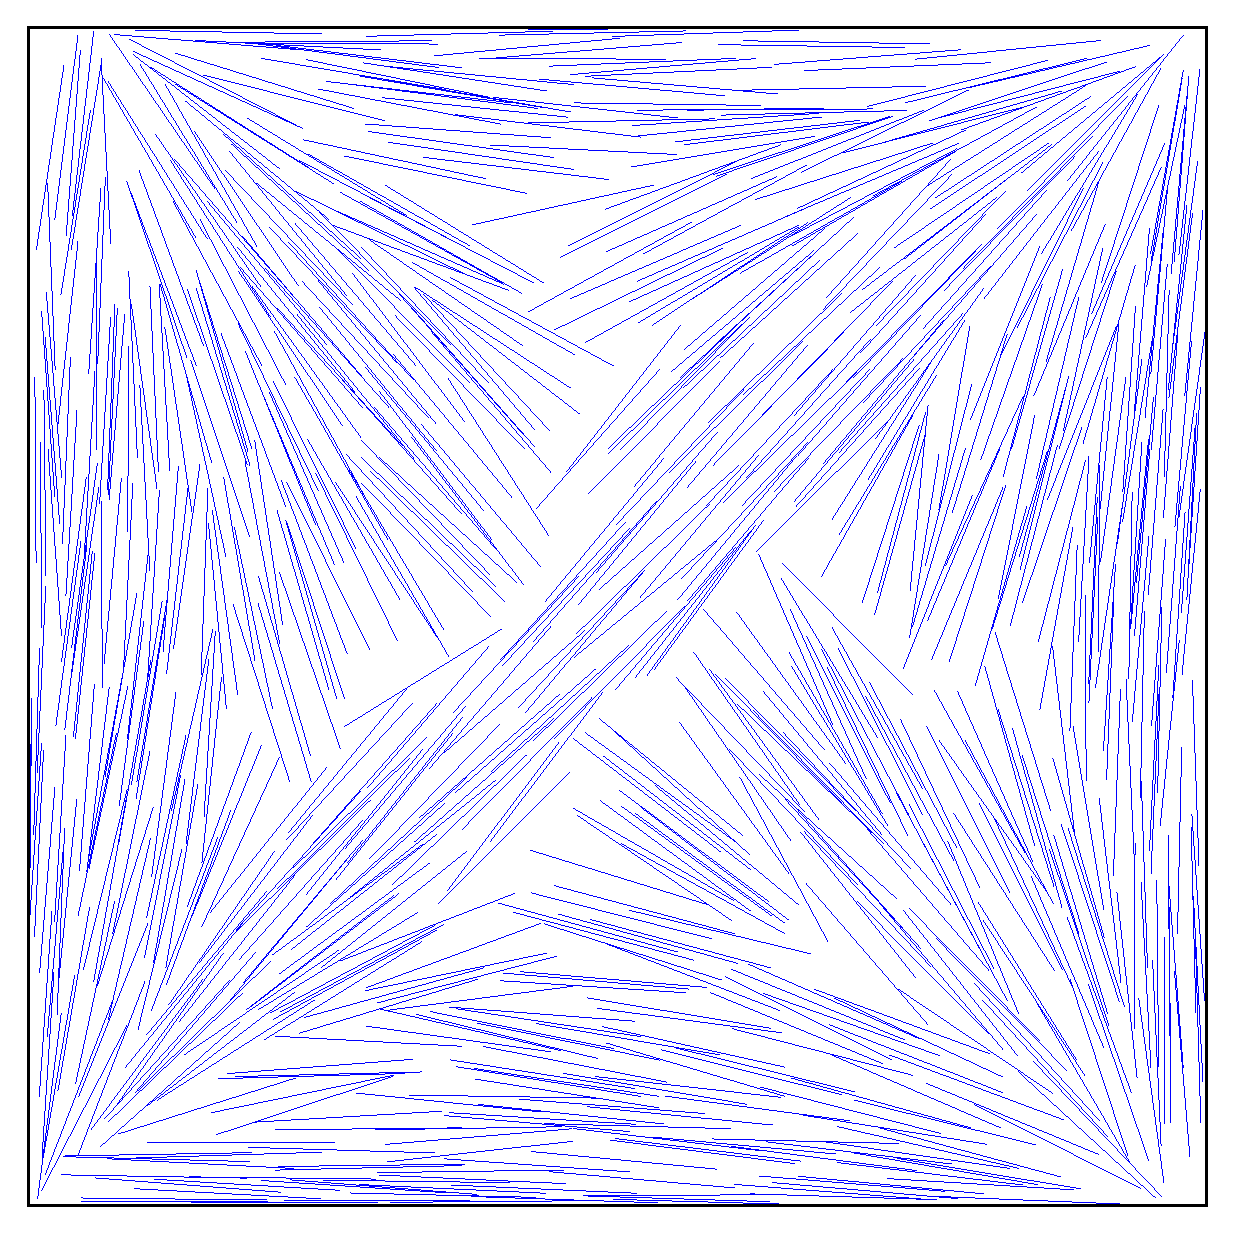
\includegraphics[width=0.9\columnwidth]{./figs/FIG1H.eps}\\
		(h)
	\end{minipage}%
	\caption{(a)-(d) Illustration of a two-dimensional hand-written image, Ising model, nematic state, and coordinates for a rodlike molecule,
		as well as (e)-(h) example configurations of different defect states generated from
		Monte Carlo simulations for a
		confined rodlike nematic fluid.
		The parameters used to generate these example configurations are $[N,L/a]=[784,6.32]$.
		The defect state in (e) has a diagonal (D) pattern, and
		the nematic textures in (f)-(h) resemble the tilted letter T, letter U, and letter X. 
	}
	\label{FIG1}
\end{figure*}

One of the simplest neural networks is the feedforward neural network (FNN). A powerful tool, FNNs are able to accomplish a variety of image recognition tasks \cite{schmidhuber_deep}, a frequent benchmark test being the MNIST hand-written digit data set \cite{mnistset}. Figure \ref{FIG1}(a) shows one such digit from the MNIST set. Increasing the size and depth of a network boosts its ability to learn more complex patterns and features contained in images and then recognize these learned patterns in a new image.
An extension of the FNN, the convoluted neural network (CNN), has the network structure organized in such a way that local features of a pattern are dissected \cite{cnnmnist}.
CNNs have thus been a natural choice for condensed matter research, in particular problems on lattices such as the Ising model \cite{carras}, the XY model \cite{beach}, correlated fermions \cite{broecker,chng}, and other quantum systems.

In condensed matter physics we often deal with ordered states, where
certain physical features display spatial correlations in long range. Two typical examples are shown in Fig.\ \ref{FIG1}. In the ferromagnetic state, within an ordered domain spins align in one direction, as illustrated in Fig \ref{FIG1}(b). In the nematic liquid crystal state, within an ordered domain molecular directions are all aligned towards a common angle [Fig \ref{FIG1}(c)].
The images produced in these examples can come from computer simulations, e.g. Monte Carlo simulations (see Appendix A for the current liquid-crystal system).
%%FNNs and CNNs are effective tools for identification of the disorder-to-ferromagnetic transition in the Ising model \cite{carras} and the isotropic-nemetic transition in the liquid crystal model [see Appendix B], when trained to recognize these different states.
Here, an ``image'' used for network learning is not a graphic image in the conventional sense. Rather, it is represented by the system configuration data containing physical features of each molecule (values of spins, angles specifying the orientations, etc).

These ordered states, on the other hand, sometimes have topological defects in their substantially ordered background. Different patterns can be characterized by different ways in which the local order parameters around the defects couple with the locations of the defects. Developing a characterization procedure to categorize these defects is a challenging task. A neural network (NN), then, becomes an ideal tool to identify these topological defects.
%In studying the Ising model with a neural network \hl{[IS THIS the paper for defect** We need to cite the defect paper here***]} \cite{carras}, an FNN was trained to recognize both high temperature (isotropic) states and low temperature (ferromagnetic) states. To read a given instance the neural net was given an ordered list of spins, from top-left to bottom-right. From this information alone the NN could learn the phase transition temperature, that is, it learned when contiguous regions were present or not.
%It would seem, then, the procedure is clear: a network with straightforward feeding of configurations through the input layer should enable the identification of defects in ordered states.
In studying the Kosterlitz-Thouless transition of the XY model \cite{beach}, a multilayered  network was trained on raw orientational configurations to learn the vortex unbinding that marks the transition. Accomplishing this requires the NN to understand topological features not too unlike the liquid crystal topologies in Fig.\ \ref{FIG1}(e)-(h). It would seem then that feeding the liquid crystal configurational data in a similar fashion should enable the identification of defects in ordered states.

However, we show here that such network structures are not readily appropriate for studying defect types of {\emph{off-lattice}} problems, such as the liquid-crystal defects shown in Fig.\ \ref{FIG1}((e)-(h)).
A typical configuration file generated from the computer simulations has a single-line data structure $[l,x_l,y_l,\theta_l]$ for a given molecule, where $l$ is the label of a molecule, and $[x_l,y_l, \theta_l]$ specify its $x$- and $y$- location coordinates and angular orientation [see Fig \ref{FIG1}(d)].
Because the molecules are allowed to randomly move in space, the label of a molecule, $l$, has no relationship at all with the spatial coordinates [see Fig \ref{FIG1}(c)].
This can be contrasted with a simulated data file produced by a lattice-model. In such a case, positional information is already embedded in the order in which molecules are labeled (one naturally reads the data in the same order every time), as demonstrated by the arrow in Fig.\ \ref{FIG1}(b).
An NN that attempts to capture position-correlated patterns is thus implicitly aided from this direct mapping of physical position to the ordering of data in a lattice model.

Hence, we must solve how to capture the main features in a topological-defect state when the correlation between defect positions and the physical properties around them is the vital property. In this paper we discuss different ways of incorporating existing NNs for this purpose. As it turns out, an FNN (and conceivably a CNN) finds correlation between the order of appearance of data in the input and the physical features to be correlated. Hence, FNNs and CNNs  can identify defect states resultant from the Ising model since the ordering of data already represents the spin positions. On the other hand, in an off-lattice model, $l$ has no correlation with  $[x_l,y_l, \theta_l]$. Even if we use $x_l, y_l$ as an input together with $\theta_l$, an FNN cannot find the correlation between $l$ and the input features $[x_l,y_l, \theta_l]$. This is discussed in Sect. \ref{FNN}.

Can we re-connect a relationship between $l$ and $x_l, y_l$ that can be easily used by an FNN for an off-lattice dataset? In Sect.
\ref{FNN} we develop and discuss a coarse-graining method which cuts the original simulation box into $m\times m$ equally sized cells where $m=1,2,4,8..$. The NN input is then ordered by cell index $M$, with the information inside each cell unordered. By such means, it is as though the system is approximated to a lattice form, with increasing accuracy as the cells become smaller and more numerous. An FNN can then begin to correlate physical features with position and identify topological defects with appropriate cell size.

However, we present another more general method, using a recurrent neural network (RNN), that avoids the need for any presorting.
The RNN is a neural network specialized in correlating sequential information (e.g.\ analyzing a time series of images \cite{rnnvideo}, or predicting upcoming words in a sentence based on previous words \cite{rnnwords1,rnnwords2}). In Sect. \ref{RNN}, we propose a scheme to feed
$x$, $y$, and $\theta$ data sequentially, akin to three time sequenced images, which enables the RNN to correlate these three features. Turning temporal correlation to spatial correlation, an RNN can efficiently identify topological defects in the original raw data, without any of the coarse-graining or presorting needed for the FNN.

We selected the topological defects appearing in the system of $N$ rodlike molecules confined by a square boundary in two dimensions (2D) as a
vehicle to deliver some of the concepts in this paper. This system has been the focus of recent theoretical and experimental studies due to its practical relevance \cite{Galanis2006,Mulder2011,Lewis2014,Cortes2017} and interesting theoretical aspects \cite{Tsakonas2007,Luo2012,chen2013rods,Mulder2015,Lewis2014}.
% above sources pulled from Yao fig 6 (earlier version)
In Ref. \cite{yao}, this system was studied in-depth, producing an ensemble of stable and metstable states. Our aim here is not a detailed study of this particular liquid crystal system, which has been done in the above listed references.
Rather, the system gives us the four major defect states, D, T, U, and X, shown in Fig.\ \ref{FIG1}(e)-(h), which we can use as examples in our machine learning study. The computer simulation procedure, as well as the system's isotropic-nematic transition properties, are explained in Appendices \ref{MC} and \ref{IN}.

Returning to the classic example of identifying hand-written numerical digits from 0 to 9, we make a comparison between the darkened pixels in this case with the topological defects in our confined liquid crystal system. In a sense, what a neural network looks for is the feature correlation of the spatial position of the darkened pixels in these images. In Appendix \ref{AppMNIST}, we re-enforce some of our concepts mentioned above, by treating the digit recognition problem as a defect identification problem.
%When it comes this classical application the question must be asked: To order or not to order?

This work is motivated by the question of whether machine learning can be used to identify topological defects, which in this case are those of confined two-dimensional liquid crystals. We clearly make recommendations on data handling and
the choice of neural network, suitable for defect identification; these can form useful steps for  more general problems in studying other condensed matter systems, in particular, data generated from off-lattice models.




\begin{figure}
\centering
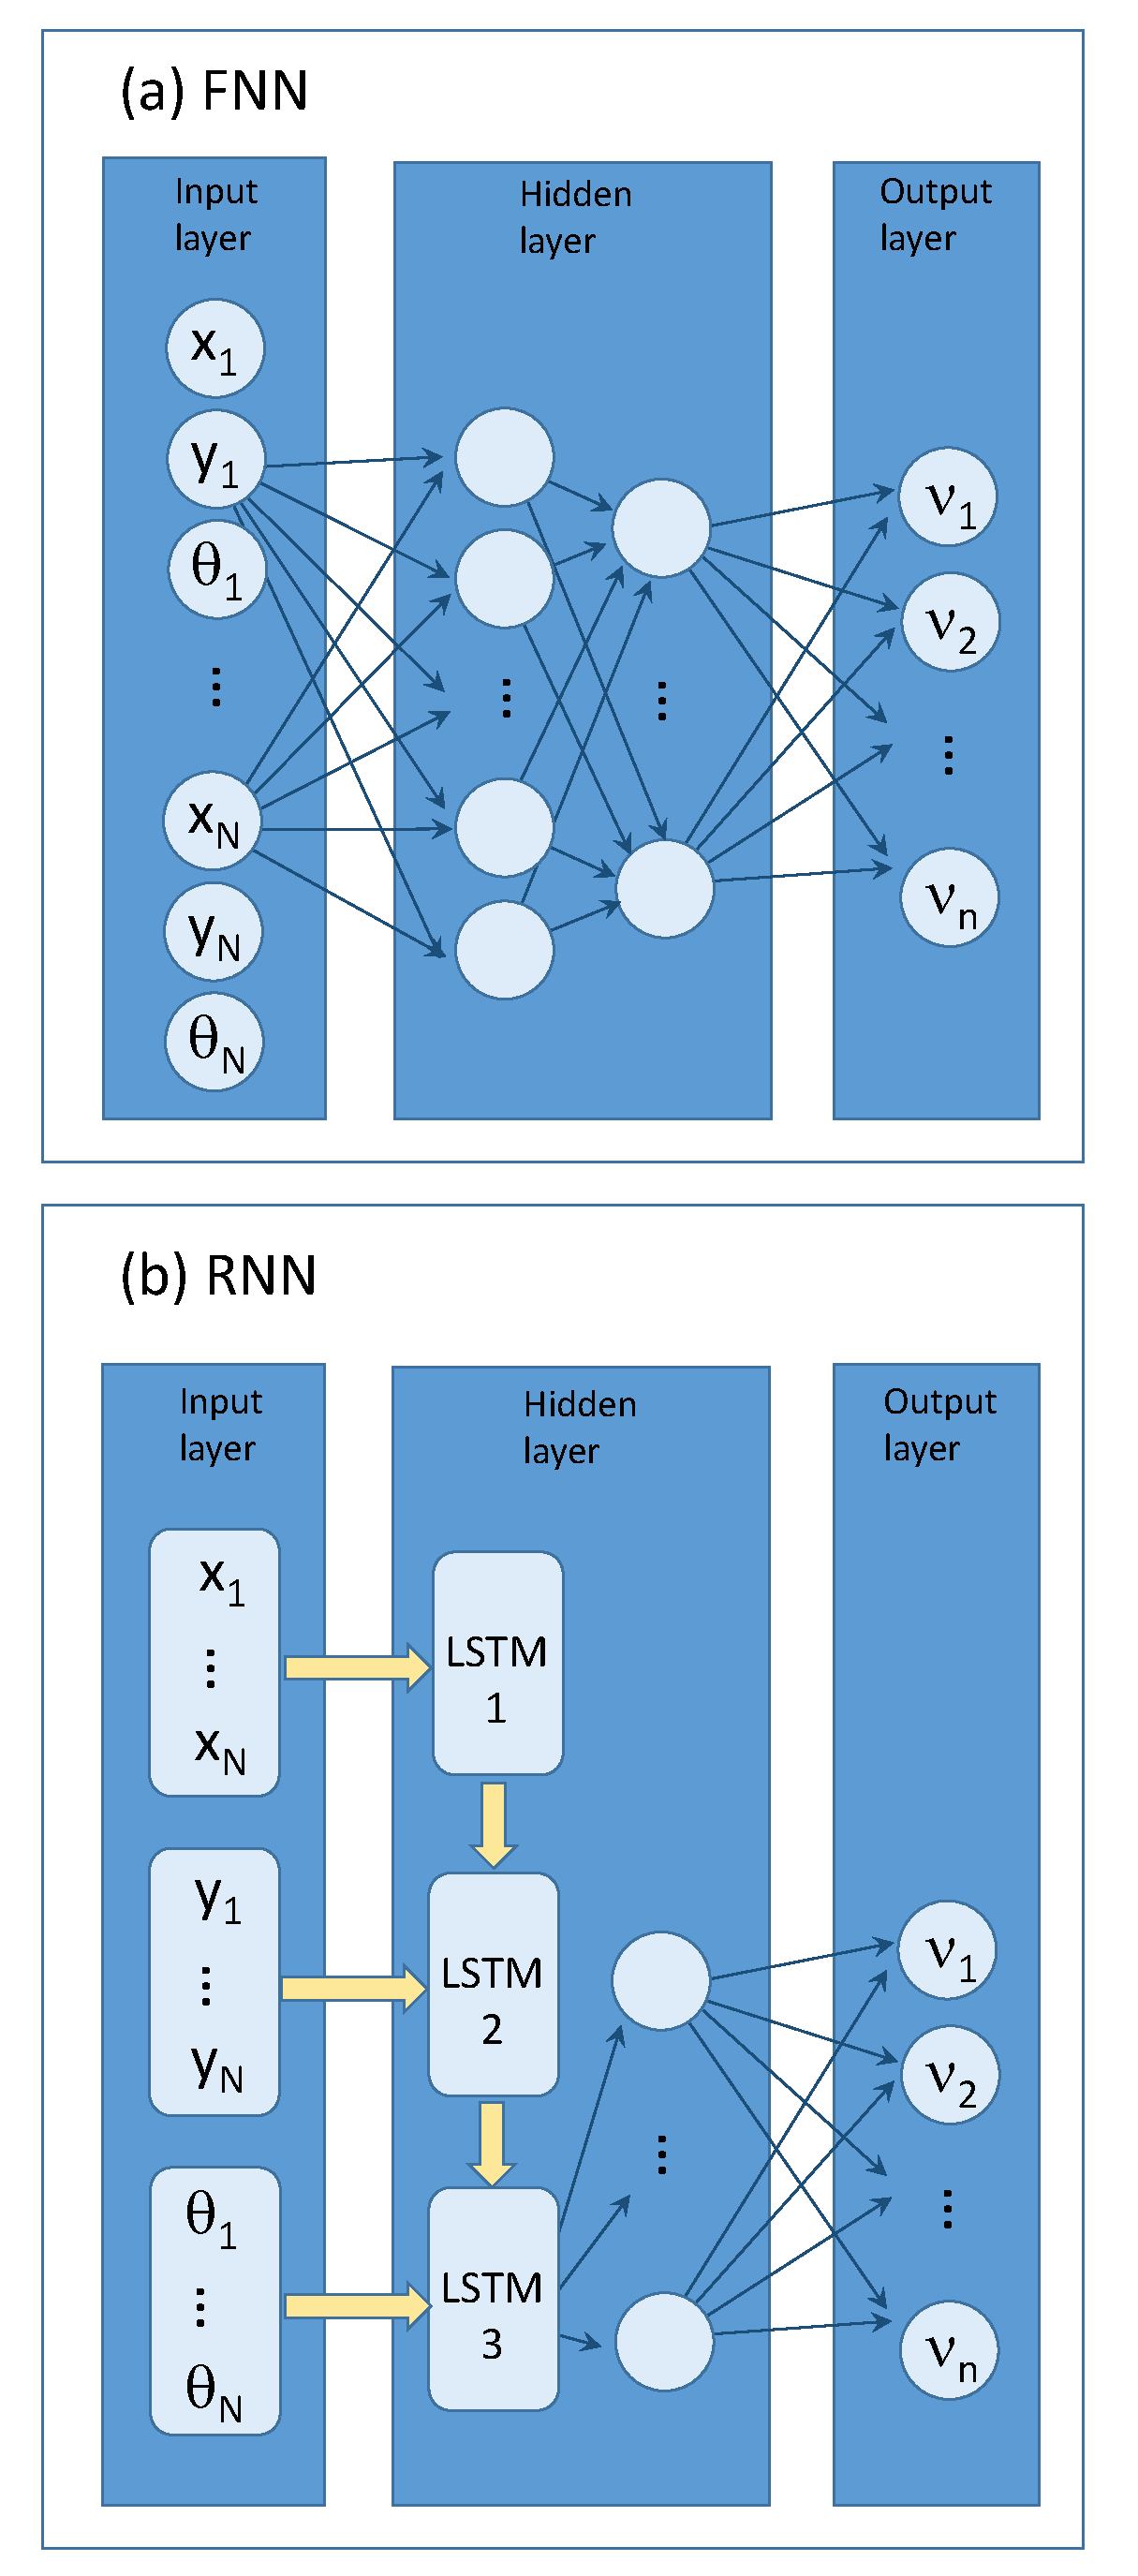
\includegraphics[width=0.5\textwidth]{./figs/FIG2.eps}
\caption{Schematics of (a) an FNN with two hidden layers and the sequence $(x_l, y_l, \theta_l)$ as input, where $l=1,2,...N$, and (b)
an RNN (unrolled) with the sequence $x_l$ ($l=1,2,...N$) as the input to the first LSTM block,
$y_l$ ($l=1,2,...N$) to the second LSTM block, and $\theta_l$ ($l=1,2,...N$) to the third LSTM block.
LSTM blocks also have LSTM-LSTM connections.
The final output of the two networks are $\nu_1, \nu_2, ..., \nu_n$, where $n$ is adjusted according to the type of features to be identified.}
\label{FIG2}
\end{figure}



\section{Application of FNN}\label{FNN}

First we review a few basic neural network concepts.
The main function of an NN is to read the system configuration through an input layer (e.g.\ an image, text, or sound bite), process the information in  hidden layers, and then generate an output. The output is often a classification estimation of the input, but may be another data structure (another image or sound bite for instance). In our case we look to classify system states through an FNN, sketched in Fig. \ref{FIG2}(a).
Each arrow (an ``edge'') represents a function call that connects nodes in different layers. These nodes, or ``perceptrons'', are inspired by the neuron model of the brain and are the building blocks of many neural networks, including the FNN, and though individually quite simple, complex functions can be represented by networking many perceptrons together \cite{rosenblatt}.
Going from input to output, data is repeatedly manipulated through function calls at each layer, with each containing their own network parameters --- usually referred to as weights and biases.
By varying network parameters the final output is consequently affected.
Training a network then involves optimizing the network's performance in producing the desirable output with respect to these network parameters.
%Multiple ``epochs'' are needed during the training, where w
Within one ``epoch'' the network is trained once on the selected dataset, and in general multiple epochs are needed for a network to converge to an acceptable performance.

A few technical details are provided.
We used a multilayer perceptron FNN of modest size, having two hidden layers: the first of size 128, and the second of size 32.
With the implementation of Tensorflow, exponential linear units were the chosen neurons for their proven effectiveness and quick learning \cite{elu,tensorflow}, and an early stopping technique determined sufficient training time \cite{nntricks}. Dropout was used at a 50\% drop rate to reduce overfitting the training \cite{dropout}.
The Adam algorithm was used for optimization \cite{adam}, and Softmax was applied to the output neurons to normalize the output set [see Appendix \ref{Supervise}].
For evaluating NN performance, a separate test dataset of images not seen during training is needed. A useful NN model needs to be able to correctly classify images it has not been trained on, otherwise it may merely have found a set of parameters that only work for the training set.

We used cross entropy $S$ as the cost function to measure the training quality on the training data set;
plotted as a function of epoch, we can see how the model learns over time and estimate its learning trajectory.
When the network is adequately trained, $S$ approaches 0. Another unique insight into the network's performance is the accuracy $A$, defined to measure the network performance on the unseen test set. An accuracy of 1 is scored for correct classification on the entire test set. Both $S$ and $A$ are quantitatively defined in Appendix \ref{Supervise}.

The physical system studied here is the defect states generated from the MC simulation of a two-dimensional off-lattice liquid-crystal model. In total, $N=784$ rod-like molecules of length $L$ are confined to a square box of dimensions $a\times a$. One can show that the parameter that drives the phase transition is the reduced density,
\begin{equation}\label{rho}
    \rho \equiv \frac{NL^2}{a^2}.
\end{equation}
Above the critical value $\rho^*$ the system is in a nematic state with directional ordering and below the critical value the system is in an isotropic state with random orientations (except those near the walls). The critical density $\rho^*\simeq 6.71$ can be estimated from a typical machine learning application, described in Appendix \ref{IN}.

\begin{figure}
\centering
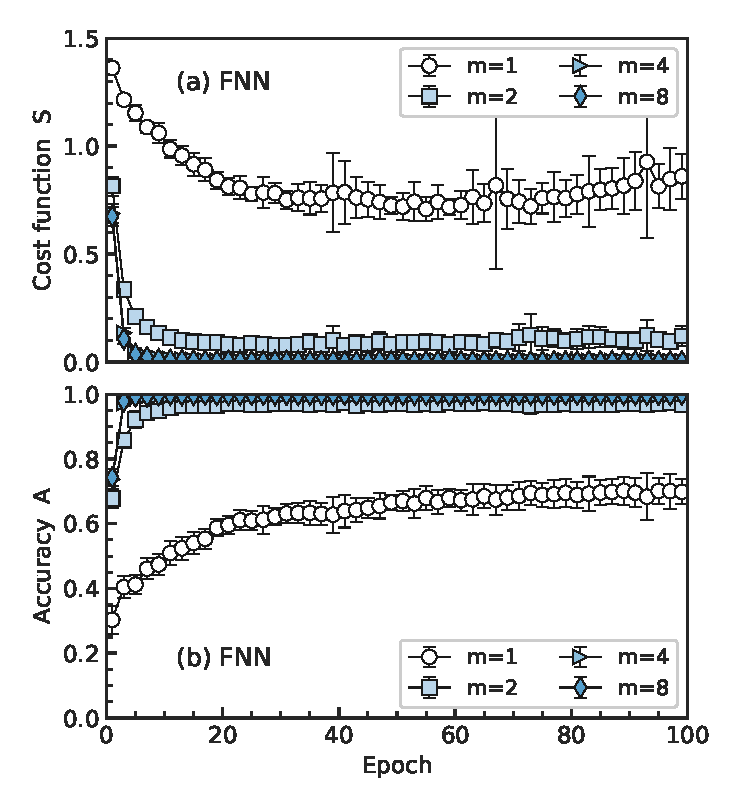
\includegraphics[width=0.8\textwidth]{./figs/FIG3AB.eps}
\caption{Cost function $S$ and accuracy $A$, defined on the training and test datasets respectively, monitored on an FNN as functions of epoch step. Symbols in the plots represent the averaged $S$ and $A$ produced from 20 repeated training runs, from which errorbars are also estimated. Circles, squares, triangles, and diamonds correspond to the degrees of coarse-graining in the presorting procedure used: $m=1$ (unsorted raw data), $2$, 4, and 8, respectively. For coarse-graining, the original simulation box in Fig.\ \ref{FIG1}(e)-(h) is divided into $m\times m$ cells [see Section \ref{FNN}].
}
\label{fnn_SA}
\end{figure}

\begin{figure}
\centering
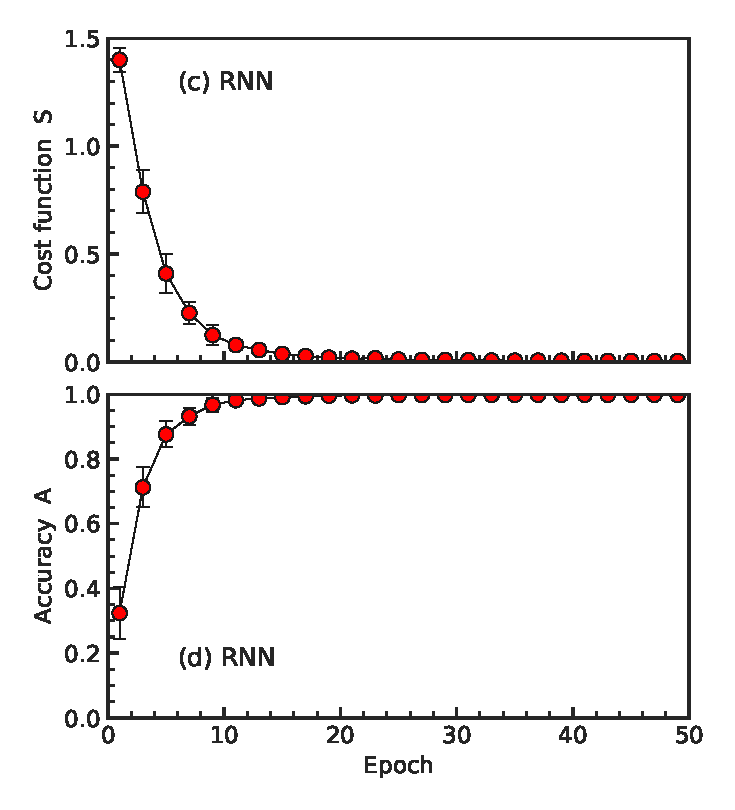
\includegraphics[width=0.8\textwidth]{./figs/FIG3CD.eps}
\caption{Cost function $S$ and accuracy $A$, defined on the training and test datasets respectively, monitored an RNN as functions of epoch step. Symbols in the plots represent the averaged $S$ and $A$ produced from 20 repeated training runs, from which errorbars are also estimated.
}
\label{rnn_SA}
\end{figure}

Our main concern here is identifying the defect states, not the isotropic-to-nematic phase transition itself.
Within the nematic state, the system can display a stable D-defect pattern, or can be trapped in the free energy minima corresponding to one of the X-, T-, or U-defect patterns, due to the finite confinement effects. The nature of the metastability has been recently addressed extensively in Refs.\ \cite{Galanis2006,Mulder2011,Lewis2014,Cortes2017,Tsakonas2007,Luo2012,chen2013rods,Mulder2015}.
In order to explore the best machining learning techniques in identifying the defect states, we established a database from the MC simulations at a fixed  $\rho=19.63$ (produced by setting $a=6.32L$). The relatively high $\rho$  enables the trapping of the metastable defect patterns during simulation runs. In total, $4400$ independent configurational snapshots were collected for each of the defect states [see Appendix \ref{MC}].
%
%To build up datasets a relatively high density of $\rho=19.63$ was used so the different defect patterns could maintain their form as they are metastable at lower densities. For each pattern $4400$ independent snapshots were collected [see Appendix \ref{MC}].
For each configuration, $4000$ were used for training and the remainder for testing. The raw dataset of each snapshot contained data ordered by the label of molecules, $l$, and followed by $[x_l,y_l,\theta_l]$.

%The MC parameters for the DTUX sets were chosen so as to be in a favorable region for both $U$ and $T$ states, as predicted by Yao \cite{yao}. We chose a box size of edge length $a=6.32$, rod length of unity, and number of rods $N=28^2$, yielding a reduced density $\rho^*=19.63$. This region, though favorable, was still only metastable and relaxing for much longer than $10^5$ Monte Carlo sweeps (where one sweep attempts to move each rod) would inevitably tend towards the more preferred D state. In accounting for this, after $10^5$ sweeps, the state snapshot would be recorded, the system would be reinitialized, and the process would repeat. This additionally ensured no temporal correlation among snapshots.

A naive approach would be directly taking an FNN for identifying these defect states, feeding the raw $[x,y,\theta]$ data into the $3N$ input nodes, and training the network to recognize the four different topologies by supervised learning [see Appendix \ref{Supervise}].
This approach has seen success in learning phase transitions of Ising systems \cite{carras}, polymer systems \cite{wei}, and the XY model \cite{beach}. However, this method showed a pronounced failure in the current application.
As we show in Fig.~\ref{xtud-all}(a), indicated as $m=1$, this approach does not come close to an acceptable performance, producing a plateau in an undiminishing cost. In addition, $A$ reaches a plateau at an unsatisfactory level of approximately $60\%$.

Why is this so?
One of the essential features the network needs to learn for these defect configurations is the correlation between the position of a topological defect and the molecular orientation in the vicinity of the defect. A typical raw snapshot datafile records the $[x,y,\theta]$ data sequentially according to the order of the label of the rodlike molecules $l$. Because there is no a priori knowledge of which molecules show up in the defect regions, the labels of the defect-region molecules differ from file to file. Indeed, in a statistically independent set of files, such as the ones produced here from different initial conditions [see Appendix \ref{MC}], there are no label-position correlations of the defect-region molecules among the learning data files.
This all addresses a crucial, but often unnoticed, aspect of image classification: by filling input vectors in a positionally sorted fashion [Fig.~ \ref{FIG1}(a),(b)], positional information, and indeed its correlation to whichever feature is being written to the input vector, is consequently encoded. If this sorting is destroyed, even if we give the positions (such as $[x,y]$
) as part of the input data, the position-feature (e.g.\ $\theta$) correlation is destroyed. This unseen property, and its essential importance can also be demonstrated via the digit recognition problem in Appendix \ref{AppMNIST}.

Hence, the key information is the position sorting in the initial data input, as the FNN relates features with the ordering of the input data. We develop the following coarse-graining procedure to train an FNN in identifying liquid crystal defects shown in Fig.~\ref{FIG1}.

The confinement box (Fig.~\ref{FIG1}) is divided into $m\times m$ cells, where $m$ is an integer. The cells are labeled $M=1,2,...m\times m$ horizontally, row by row.
The raw data in every snapshot is presorted according to their $[x,y]$ coordinates so that molecules belonging to the $M=1$ cell show up first, $M=2$ cell show up second, etc. Within a cell, the order of data is still random and no further presorting is made. The $m=1$ case returns to the raw data format. By the end, the order of appearance of molecular information is no longer according to $l$, but, according to $M$ for all coarse-graining degree $m\ge 2$. The presorted data is then used in supervised training.

The presorting procedure works well with an FNN. Figures \ref{fnn_SA}(a) and (b) show how the cost function and accuracy quickly approach the ideal value of $0$ and $1$ respectively, as we presort the data beyond $m=2$.
In the case of $m=4, 8$, less than 20 epochs (surprisingly short) are needed to adequately train the FNN. This can be attributed to the defect patterns in Fig.\ \ref{FIG1} themselves. By dividing the square box in $m=4$ cells, for example, one can already distinguish the defect structures, by ignoring fine details inside a single cell.
Of course,  in general we expect that the degree of coarse-graining, $m$, needs to increase for a more complicated defect pattern with more defect features.

In summary, to effectively train an FNN to identify features in an image or simulation data file, the ordering of data points (pixels in image, spins in the Ising model, and rodlike molecules in the current study) contains vital information of the data. An off-lattice model usually produces data with a random order and it must be presorted according their approximate $[x,y]$ coordinates, if we are looking for the correlation between coordinates and the physical features.

\section{Application of RNN}\label{RNN}

A typical structure of the recurrent neutral network (RNN) is represented in Fig.~\ref{FIG2}(b). The crux of this RNN is the long short-term memory (LSTM) cell module \cite{lstm}. An RNN can be made with different types of modules, but LSTM is a popular choice and is well-sufficient for this work. Except for the first block, an LSTM cell has two input channels: an LSTM-external connection
to new raw data from the system to be studied,
and an LSTM-LSTM connection, taking its own output and internal weights from the previous step as input, hence the recurrent aspect. Schematically, it helps to show a series of LSTM cells for each raw data input. %, but there is really only one.
To complete the RNN, a single layer of perceptrons is appended to act as
a final interpretive layer of the LSTM output, which compresses the large LSTM output to the smaller prediction output $(\nu_1, \nu_2, ..., \nu_n)$.

A typical application of an RNN is comparing a time series of data.
An LSTM cell can take a complete data file and at each iteration of input, consider the new raw data together with its own previous state simultaneously. That is, an LSTM establishes data correlations with those fed into earlier cell states through LSTM-LSTM connections.
%A popular application of RNNs is speech recognition, where a long series of connected LSTM blocks are used; if one uses $i$ to denote LSTM blocks sequentially, then the input to the $i$th LSTM block is a complete dataset occurred at time frame $t_i$; the time series $...t_{i-2}, t_{i-1}, t_i$ of a speech record can then be processed with time-correlation.
In its composition, like an FNN, an RNN (including the LSTM) is still merely an ensemble of floating-point network parameters.
The logic of supervised training is the same here in comparison with an FNN: determination of the network parameters through optimization of a cost function. The RNN can be coded in terms of Tensorflow libraries efficiently.


Here we demonstrate a novel usage of an RNN in condensed matter systems. Exploiting its ability to correlate physical features through LSTM blocks, we adopt a triple iterative structure shown in Fig.\ \ref{FIG2}(b) to find the correlation between the spatial coordinates $x$, $y$ and the orientational coordinate $\theta$. The raw data
has a line-by-line format $[l, x_l, y_l, \theta_l]$, where $l=1,..., N$. The three main features, $x_l, y_l$ and $\theta_l$ are input into the network model iteratively through the LSTM-external layer, one after another. As a technical note, we used a rather small RNN having only a single layer LSTM of 64 hidden neurons, and a single perceptron layer of 128 neurons. Dropout, Adam optimization, and early stopping were again used throughout the supervised training \cite{dropout,nntricks,adam}.

The performance of this RNN is exceptionally good in identifying the defect states. Figures \ref{rnn_SA}(c) and (d) demonstrate that within an initial 20 epochs, our RNN efficiently captures the main features of the four defect states, evaluated on an unseen test dataset. We stress here that unlike the procedure used to produce Figs. \ref{fnn_SA}(a) and (b), we used the raw, unsorted data as the input on our RNN experiment.

%It is not surprising because RNN is known to capture temporal correlations, and it is adopted here to capture spatial correlations.


%The correlation is achieved thanks to the sequential feeding of the $x,y$, and $\theta$ features. Like the FNN, the LSTM has an internal set of weights that are trained while optimizing the model. While reading the sequence of inputs, the LSTM also maintains a ``cell state''. This cell state is updated with each input, first on the $x$ data, again on the $y$ data, and a third time on the $\theta$ data. Additionally, updating the cell state not only depends on what current information is being fed, but also on the previous cell state (hence the recurrent attribute). For example, we may consider two images that have the same value $\theta_i$ in the $i$th position (or even an identical $\theta$ vector) but different $[x_i,y_i]$ coordinates. The structure of the RNN naturally correlates $\theta_i$ to the position coordinates also in their $i$th positions and so interprets the angular information properly.
